\documentclass{article}

\usepackage{graphicx}
\usepackage{tikz}
\usepackage{tikzsymbols}
\usetikzlibrary{calc,patterns,shapes.geometric}
\pagestyle{empty}
\usepackage[margin=0pt]{geometry}
\geometry{papersize={14in,12in}}

\def\centerarc[#1](#2)(#3:#4:#5){\draw[#1] ($(#2)+({#5*cos(#3)},{#5*sin(#3)})$) arc (#3:#4:#5);}

\begin{document}
	\begin{figure}
		\centering
		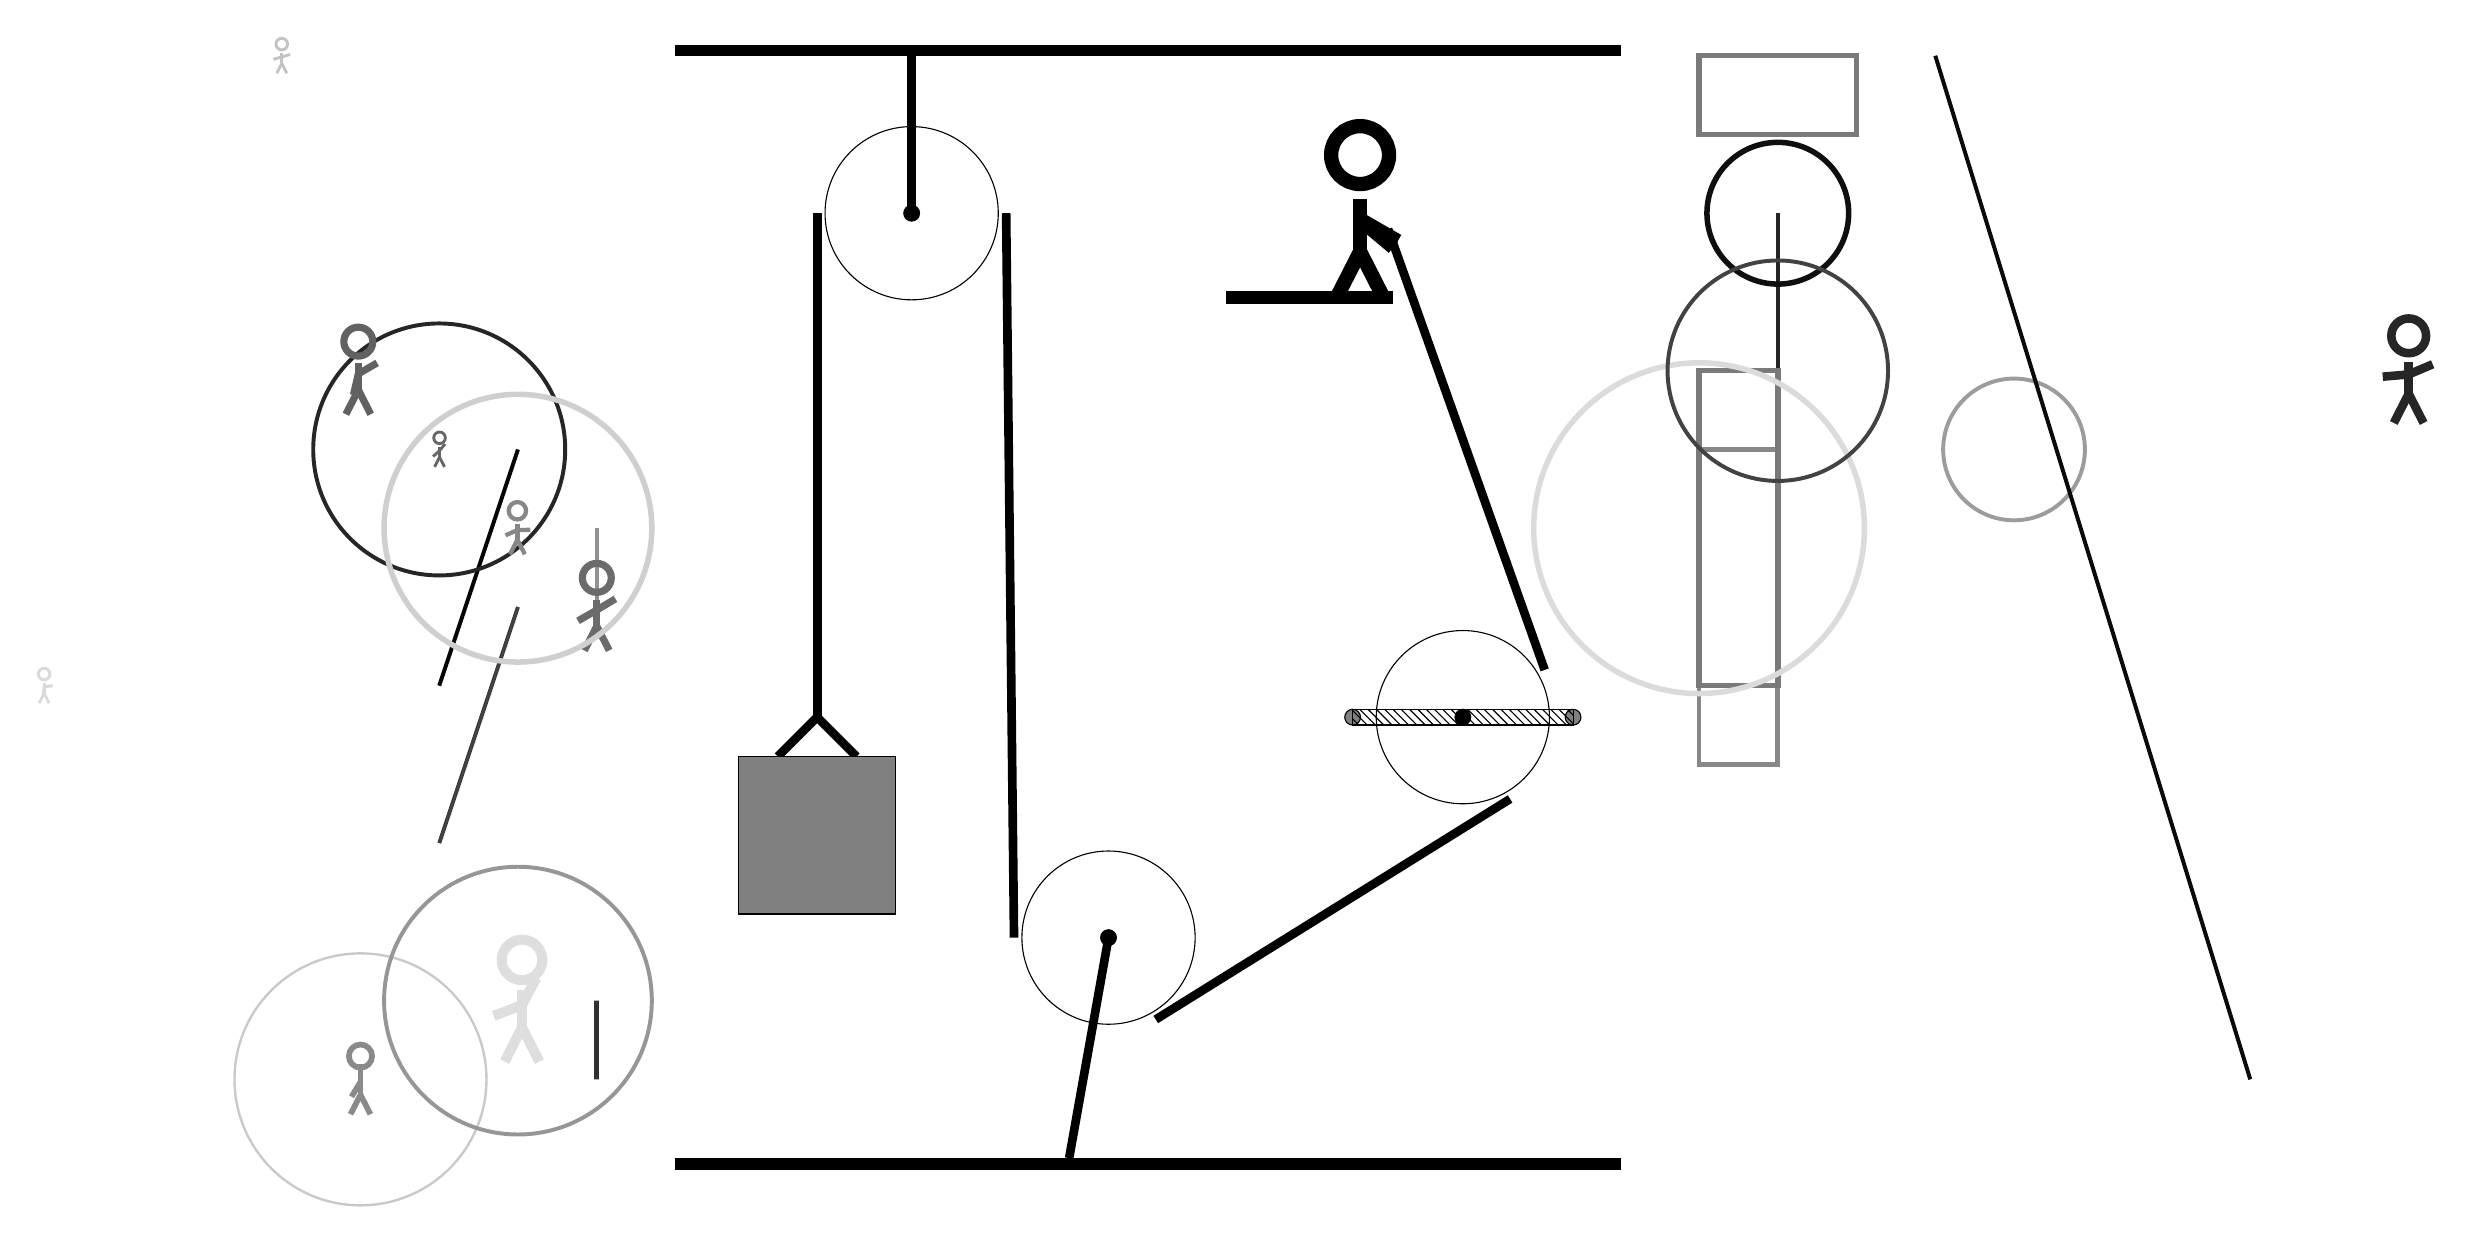
\begin{tikzpicture}
			%%%%% START %%%%%
			
			\draw[fill=black] (-2, 14) rectangle (10, 14.125);
			
			\draw (1, 12) circle (1.1);
			\draw[fill=black] (1, 12) circle (0.1);
			\draw[line width=1.1mm] (1, 14) -- (1, 12);
			
			\draw (3.5, 2.8) circle (1.1);
			\draw[fill=black] (3.5, 2.8) circle (0.1);
			\draw[line width=1.1mm] (3.5, 2.8) -- (3.0, 0);
			
			\draw[fill=white](8, 5.6) circle (1.1);
			\draw[fill=black] (8, 5.6) circle (0.1);
			\draw[fill=black!50] (9.4, 5.6) circle (0.1);
			\draw[fill=black!50] (6.6, 5.6) circle (0.1);
			\draw[pattern=north west lines, pattern color=black] (6.6, 5.7) rectangle (9.4, 5.5);
			
			\draw[line width=1.1mm](-0.7, 5.1) --  (-0.2, 5.6) -- (0.3, 5.1);
			\draw[fill=black!50] (-1.2, 5.1) rectangle (0.8, 3.1);
			
			\draw[line width=1.1mm](-0.2, 12) -- (-0.2, 5.6);
			\centerarc[line width=1.1mm](1, 12)(180:0:1.2000000000000002)
			\draw[line width=1.1mm](2.2, 12) -- (2.3, 2.8);
			\centerarc[line width=1.1mm](3.5, 2.8)(180:300:1.2000000000000002);
			\draw[line width=1.1mm](4.1, 1.7608) -- (8.6, 4.5608);
			\centerarc[line width=1.1mm](8, 5.6)(300:390:1.2000000000000002);
			\draw[line width=1.1mm](9.0392, 6.2) -- (7.05, 11.8);
			
			\draw[line width=0.5mm, color=black!99](-5, 6) -- (-4, 9);
			
			\draw [line width=0.5mm, color=black!85](-5, 9) circle (1.6);
			\draw[line width=0.5mm, color=black!86](12, 12) -- (12, 5);
			\draw[line width=0.5mm, color=black!43](-3, 8) -- (-3, 7);
			\draw[line width=0.5mm, color=black!75](-5, 4) -- (-4, 7);
			\node[line width=0.6mm, color=black!58] at (-3, 7) {\Strichmaxerl[5][30][31]};
			\node[line width=0.7mm, color=black!62] at (-6, 10) {\Strichmaxerl[5][77][30]};
			\draw [line width=0.5mm, color=black!39](15, 9) circle (0.9);
			\draw [line width=0.3mm, color=black!21](-6, 1) circle (1.6);
			\node[line width=0.4mm, color=black!15] at (-10, 6) {\Strichmaxerl[2][83][8]};
			\draw[line width=0.7mm, color=black!52] (11, 14) rectangle (13, 13);
			\node[line width=0.5mm, color=black!13] at (-4, 2) {\Strichmaxerl[7][21][62]};
			\draw[line width=0.6mm, color=black!47] (12, 9) rectangle (11, 5);
			
			\node[line width=0.6mm, color=black!47] at (-4, 8) {\Strichmaxerl[3][24][1]};
			\node[line width=0.4mm, color=black!24] at (-7, 14) {\Strichmaxerl[2][15][17]};
			\node[line width=0.5mm, color=black!85] at (20, 10) {\Strichmaxerl[6][5][23]};
			
			\node[line width=0.3mm, color=black!46] at (-6, 1) {\Strichmaxerl[4][59][90]};
			\draw [line width=0.7mm, color=black!94](12, 12) circle (0.9);
			\draw[line width=0.7mm, color=black!52] (12, 6) rectangle (11, 10);
			
			\draw [line width=0.7mm, color=black!14](11, 8) circle (2.1);
			\node[line width=0.3mm, color=black!60] at (-5, 9) {\Strichmaxerl[2][42][51]};
			
			\draw [line width=0.7mm, color=black!19](-4, 8) circle (1.7);
			
			\draw [line width=0.5mm, color=black!41](-4, 2) circle (1.7);
			\draw [line width=0.5mm, color=black!74](12, 10) circle (1.4);
			\draw[line width=0.7mm, color=black!81] (-3, 2) rectangle (-3, 1);
			
			\draw[line width=0.5mm, color=black!96](14, 14) -- (18, 1);
			
			\node at (6.75, 12) {\Strichmaxerl[10][-220][-30]};
			\draw[fill=black] (5, 11) rectangle (7.1, 10.85);
			
			\draw[fill=black] (-2, 0) rectangle (10, -0.15);
			
			%%%%% END %%%%%
		\end{tikzpicture}
	\end{figure}	
\end{document}